% This must be in the first 5 lines to tell arXiv to use pdfLaTeX, which is strongly recommended.
\pdfoutput=1
% In particular, the hyperref package requires pdfLaTeX in order to break URLs across lines.

\documentclass[11pt]{article}

% Remove the "review" option to generate the final version.
\usepackage[review]{acl2023}
% Standard package includes
\usepackage{times}
\usepackage{latexsym}

% For proper rendering and hyphenation of words containing Latin characters (including in bib files)
\usepackage[T1]{fontenc}
% For Vietnamese characters
% \usepackage[T5]{fontenc}
% See https://www.latex-project.org/help/documentation/encguide.pdf for other character sets

% This assumes your files are encoded as UTF8
\usepackage[utf8]{inputenc}
\usepackage{natbib}  % DO NOT CHANGE THIS AND DO NOT ADD ANY OPTIONS TO IT
\usepackage{caption} 
% This is not strictly necessary, and may be commented out,
% but it will improve the layout of the manuscript,
% and will typically save some space.
\usepackage{graphicx}
\usepackage{multirow,array}
\usepackage{bm}
\usepackage{bbm}
\usepackage{algorithm,algorithmicx}
% \usepackage{algorithmic}
\usepackage{amsmath}
\usepackage{amsthm}
\usepackage{verbatim}
\usepackage{booktabs}
\usepackage{amsfonts,amssymb} 
\usepackage[noend]{algpseudocode}
\newcommand{\minitab}[2][l]{\begin{tabular}{#1}#2\end{tabular}}


\newcommand{\secref}[1]{Section \ref{#1}}
\newcommand{\figref}[1]{Figure \ref{#1}}
\newcommand{\eqnref}[1]{Eq. (\ref{#1})}
\newcommand{\tabref}[1]{Table \ref{#1}}
\newcommand{\exref}[1]{Example \ref{#1}}
\newcommand{\KZ}[1]{\textcolor{blue}{Kenny: #1}}


% If the title and author information does not fit in the area allocated, uncomment the following
%
%\setlength\titlebox{<dim>}
%
% and set <dim> to something 5cm or larger.

%\title{Pruning  Pre-trained Language Models with Principled Weight Importance and Self-regularization}

% Author information can be set in various styles:
% For several authors from the same institution:
% \author{Author 1 \and ... \and Author n \\
	%         Address line \\ ... \\ Address line}
% if the names do not fit well on one line use
%         Author 1 \\ {\bf Author 2} \\ ... \\ {\bf Author n} \\
% For authors from different institutions:
% \author{Author 1 \\ Address line \\  ... \\ Address line
	%         \And  ... \And
	%         Author n \\ Address line \\ ... \\ Address line}
% To start a seperate ``row'' of authors use \AND, as in
% \author{Author 1 \\ Address line \\  ... \\ Address line
	%         \AND
	%         Author 2 \\ Address line \\ ... \\ Address line \And
	%         Author 3 \\ Address line \\ ... \\ Address line}

%\author{First Author \\
	%	Affiliation / Address line 1 \\
	%	Affiliation / Address line 2 \\
	%	Affiliation / Address line 3 \\
	%	\texttt{email@domain} \\\And
	%	Second Author \\
	%	Affiliation / Address line 1 \\
	%	Affiliation / Address line 2 \\
	%	Affiliation / Address line 3 \\
	%	\texttt{email@domain} \\}

\begin{document}
	\appendix
	\section{Preliminary Study}
	We show the accuracy-rank trade-offs on MRPC, RTE, and CoLA in \figref{fig:pre}~(CoLA is additionally included compared to the main body of the paper). The observation on CoLA is similar to MRPC/RTE: first-order unstructured pruning can extract subnetworks that are most accurate while having the lowest average matrix rank, which lays the crucial foundation of later factorization.

%\begin{theorem}
%	Let $t_i$ and $t_{j}$ where $t_{i}\geq t_{j}$ denote the time steps at which two different checkpoints are saved; Let $R(f_{\bm{\theta}^{(t\leftarrow t_i)}})$ and $R(f_{\bm{\theta}^{(t\leftarrow t_j)}})$ denote the expected generalization error of models learned from two checkpoints $\bm{\theta}^{(t_i)}$ and $\bm{\theta}^{(t_j)}$; Let n denotes the size of training data; $|\cdot|_{\text{C}}$ denotes a function class capacity measure like VC-dimension. Based on previous expositions on VC theory, the following asymptotic generalization bound holds:
%	\begin{align}\nonumber
%		R(f_{\bm{\theta}^{(t\leftarrow t_i)}})&=R(f_{\bm{\theta}^{(t\leftarrow t_i)}})-R(f_{\bm{\theta}^{(t_i)}})+R(f_{\bm{\theta}^{(t_i)}}) \\ \nonumber
%				&\leq O(\frac{|f_{\bm{\theta}^{(t)}}|_{\text{C}}}{n^{\alpha_{i}}})+ \epsilon_{t,t_i} + R(f_{\bm{\theta}^{(t_i)}}) \\ \nonumber 
%				&=  \underbrace{O(\frac{|f_{\bm{\theta}^{(t)}}|_{\text{C}}}{n^{\alpha_{i}}}) + \underset{\bm{\theta}^{(t)}\in \mathcal{F}_{\bm{\theta}^{(t\leftarrow t_i)}}}{\inf}R(f_{\bm{\theta}^{(t)}})}_{bound(f_{\bm{\theta}^{(t\leftarrow t_i)}})} \\ \nonumber
%		R(f_{\bm{\theta}^{(t\leftarrow t_j)}})&=R(f_{\bm{\theta}^{(t\leftarrow t_j)}})-R(f_{\bm{\theta}^{(t_j)}})+R(f_{\bm{\theta}^{(t_j)}}) \\ \nonumber
%&\leq O(\frac{|f_{\bm{\theta}^{(t)}}|_{\text{C}}}{n^{\alpha_{j}}})+ \epsilon_{t,t_j} + R(f_{\bm{\theta}^{(t_j)}}) \\ \nonumber 
%&=  \underbrace{O(\frac{|f_{\bm{\theta}^{(t)}}|_{\text{C}}}{n^{\alpha_{j}}}) + \underset{\bm{\theta}^{(t)}\in \mathcal{F}_{\bm{\theta}^{(t\leftarrow t_j)}}}{\inf}R(f_{\bm{\theta}^{(t)}})}_{bound(f_{\bm{\theta}^{(t\leftarrow t_j)}})}
%	\end{align}
%where $\epsilon_{t,ti}$ is the approximation error of function class $\mathcal{F}_{\bm{\theta}^{(t\leftarrow t_i)}}$ with respect to $f_{\bm{\theta}^{(t_i)}}$. $\epsilon_{t,tj}$ is defined in analogy.
%	Because: (1) $\bm{\theta}^{(t_i)}$ is a later checkpoint with higher sparsity than $\bm{\theta}^{(t_j)}$, we have the learning speed $1\geq \alpha_{i}\geq \alpha_{j}\geq \frac{1}{2}$; (2) $\bm{\theta}^{(t_i)}$ has lower generalization error than $\bm{\theta}^{(t_j)}$, we have the following inequality holds with large probability:
%	\begin{align}\nonumber
%		bound(f_{\bm{\theta}^{(t\leftarrow t_i)}}) \leq bound(f_{\bm{\theta}^{(t\leftarrow t_j)}})
%	\end{align}
%\end{theorem}

\begin{figure*}[t]
	\centering
	\scalebox{0.285}{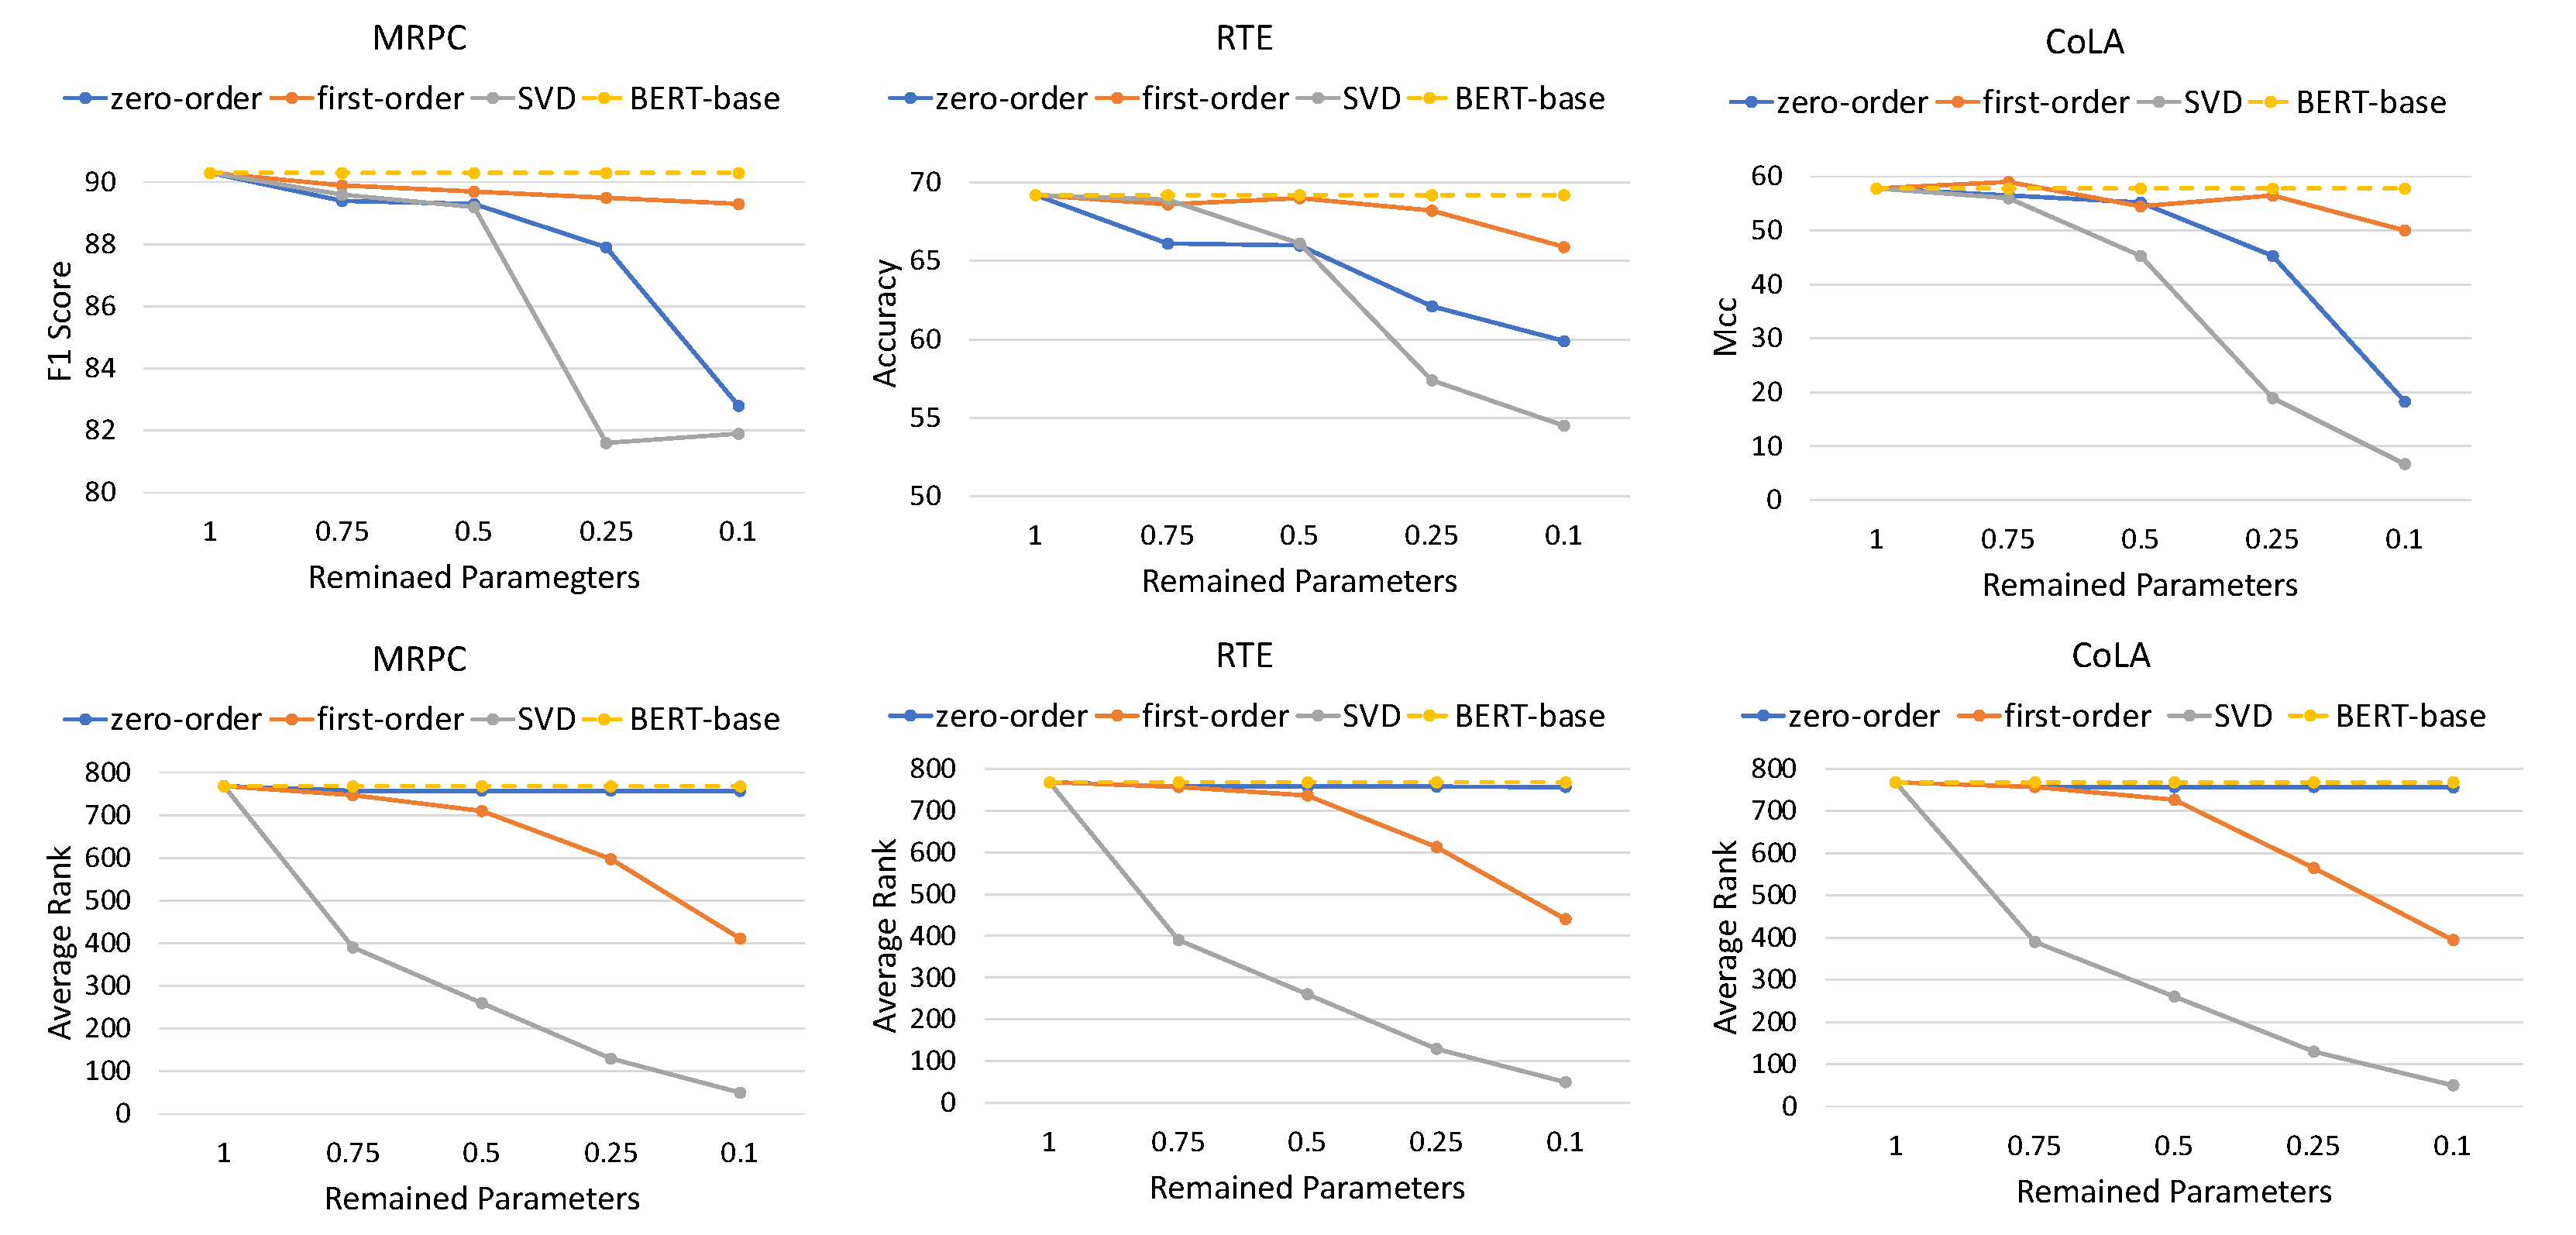
\includegraphics{./figures/pre_new.pdf}}
	\caption{Task accuracy (top half) and average matrix rank (bottom half) v.s. percentage of original parameters retained. The dashed line indicates the performance/rank upper bound by fine-tuning the full-scale BERT-base model.}
	\label{fig:pre}
\end{figure*}

\end{document}
